% change the aspect ratio to 169 for 16:9 aspect ratio
% otherwise remove option completely for 3:2 ratio.
\documentclass[aspectratio=169]{beamer}
\usepackage[utf8]{inputenc}
\usepackage{amsmath}
\usepackage{amsfonts}
\usepackage{graphicx}


\usetheme{CambridgeUS}

\useinnertheme{rectangles}

% Depending on whether you want dark or light
% theme you can change the style file, 
% drexel-light.tex for light theme and
% drexel-dark.tex for dark theme
\definecolor{drylo}{RGB}{255, 198, 0}
\definecolor{drybl}{RGB}{0,47,108}
 
\definecolor{drblk}{RGB}{0,0,0} 


\setbeamercolor{title}{fg=drybl,bg=drylo}
\setbeamercolor{subtitle}{fg=drybl,bg=drylo}
\setbeamercolor{frametitle}{fg=drybl,bg=drylo!70}
\setbeamercolor{section in head/foot}{bg=drylo}
\setbeamercolor{section in head/foot}{fg=drybl}
\setbeamercolor{subsection in head/foot}{bg=drybl}
\setbeamercolor{author in head/foot}{bg=drylo}
\setbeamercolor{author in head/foot}{fg=drybl}
\setbeamercolor{date in head/foot}{fg=white,bg=drblk}
\setbeamercolor{title in head/foot}{fg=drylo,bg=drybl}

\setbeamercolor{local structure}{fg=drylo,bg=drybl}


\author{Author Name}
\title{Sed ut perspiciatis unde omnis iste natus.}

\date{\today} 
\subject{Physics} 

% depending on dark or light theme use _black or _white pdf for drexel logo.
% These logos are obtained from https://drexel.edu/identity/drexel/logotypes/


% Two graphics side by side
%\titlegraphic{%
%    %\hfill
%    
\includegraphics[height=0.7cm]{./images/Drexel_horizontal_black.pdf}%
%    \hfill%
%    
\includegraphics[height=1cm]{./images/EXO_logo.pdf}%
%}

%%%%% Only Drexel
\titlegraphic{%
    %\hfill
    
\includegraphics[height=0.7cm]{./images/Drexel_horizontal_black.pdf}%
    %
\includegraphics[height=0.7cm]{./images/Drexel_horizontal_white.pdf}%
}


\begin{document}

\titlepage

\section{Section A}
%
%
%
%
%
\begin{frame}{Text Only Slide}{Subtitle of the slide}
    \begin{itemize}
        \item Lorem ipsum dolor sit amet, consectetur adipiscing elit
        \item Sed do eiusmod tempor incididunt ut labore et dolore magna aliqua.
        \item Ut enim ad minim veniam, quis nostrud exercitation ullamco laboris nisi ut
        \item Aliquip ex ea commodo consequat. Duis aute irure dolor in reprehenderit in voluptate velit esse cillum dolore eu
        \item Fugiat nulla pariatur. Excepteur sint occaecat cupidatat non proident, sunt in culpa qui officia deserunt mollit anim id est laborum.
    \end{itemize}
\end{frame}
%
%
%
%
\begin{frame}{Text and Image split in half} %{Subtitle not required in this slide}
    \begin{columns}
        \begin{column}{0.49\textwidth}
            \begin{itemize}
                \item Slide with figure and caption
                \item \texttt{figure} float environment used
                \item Figure \ref{fig:fig_label} shows this idea
            \end{itemize}
        \end{column}
        \begin{column}{0.49\textwidth}
            %
            \begin{figure}[h!]
                \centering
                \includegraphics[width=\linewidth]{example-image-a}
                \caption{This is caption}
                \label{fig:fig_label}
            \end{figure}
        \end{column}
    \end{columns}
\end{frame} 
%
%
%
%
%
\section{Section B}
%
%
%
\begin{frame}{Slide with Flip Images}
    \begin{columns}
        \begin{column}{0.49\textwidth}
            \begin{itemize}
                \item Two images of exact same size and resolution flip
                \item The images are not in figure environment
            \end{itemize}
        \end{column}
        \begin{column}{0.49\textwidth}
            \only<1>{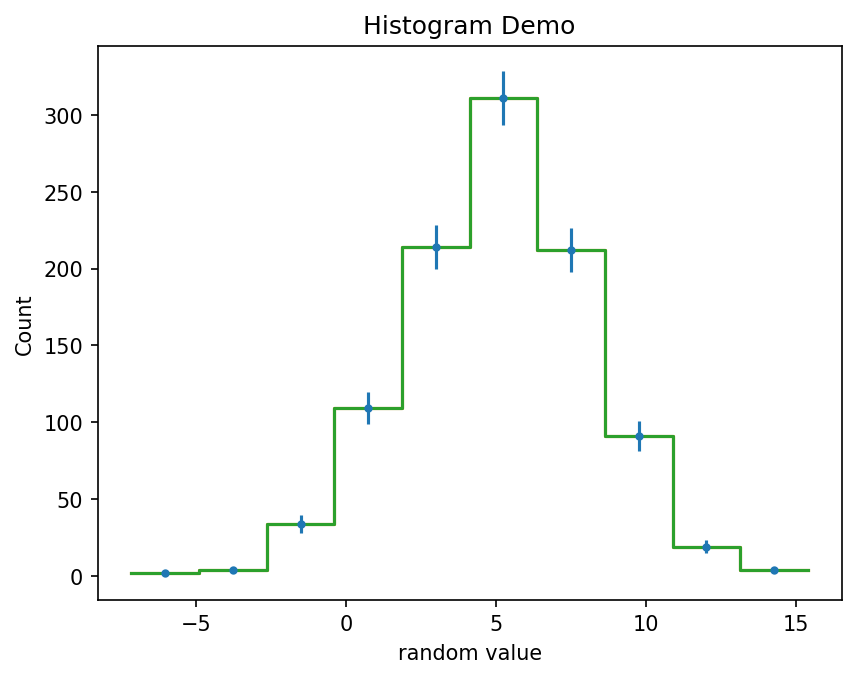
\includegraphics[width=0.98\linewidth]{./images/demo_hist_light.png}}
            \only<2>{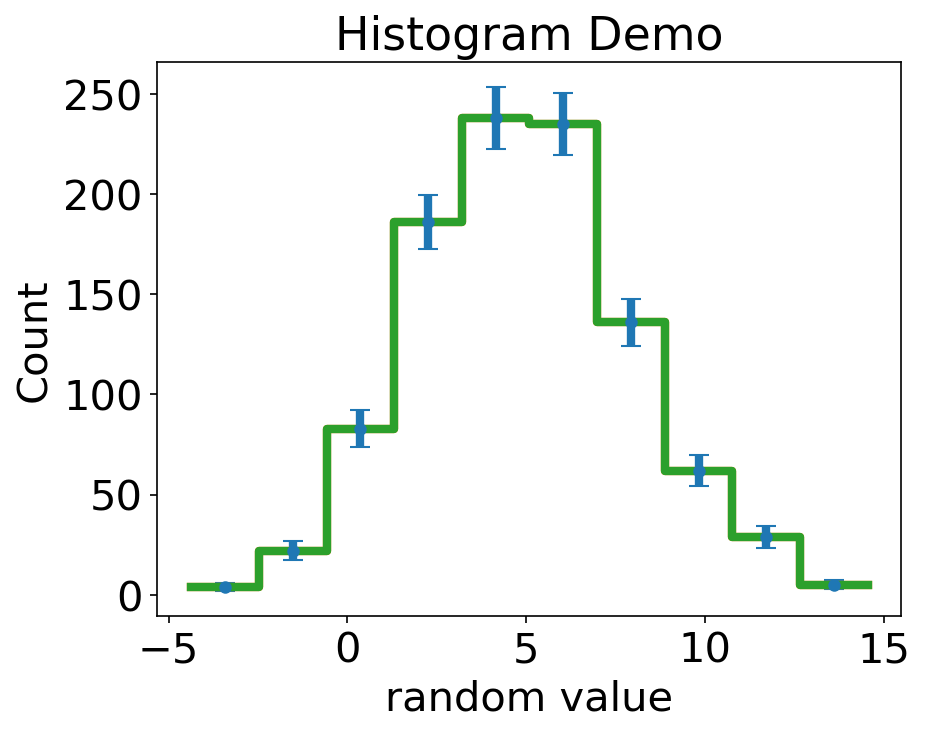
\includegraphics[width=0.98\linewidth]{./images/demo_hist_slide.png}}
        \end{column}
    \end{columns}
\end{frame} 
%
%
%
\end{document}

